\section{Reflection Substitution} \label{sec:reflectionsubstitution}

Reflection substitution is just a special case of $u$-substitution, but it's remarkably useful. We simply make the substitution $x\mapsto a+b-x$,

$$ \int_a^b f(x)\,\dx x = \int_a^b f(a+b-x)\,\dx x .$$

\subsection*{Definition}
The definition is rather easy to state as we are only making a simple substitution. Consider, $\int_a^b f(x)\,\dx x$. Let $x \mapsto a+b-x$ and $\dx x \mapsto -\dx x$.

\begin{align*}
    \int_a^b f(x)\,\dx x &= - \int_b^a f(a+b-x)\,\dx x \\
    &= \int_a^b f(a+b-x)\,\dx x
\end{align*}

\subsection*{Intuition}
Graphically the method represents a \textit{reflection} about the line $x=\frac{b+a}{2}$, depicted in figure (\ref{fig:reflectionsubstitution}). We see here that the area of the shaded region is the same for both functions. Consider the integral $$ \int_2^6 \sqrt{x}\,\dx x. $$

% a+b-x figure
\begin{figure}
    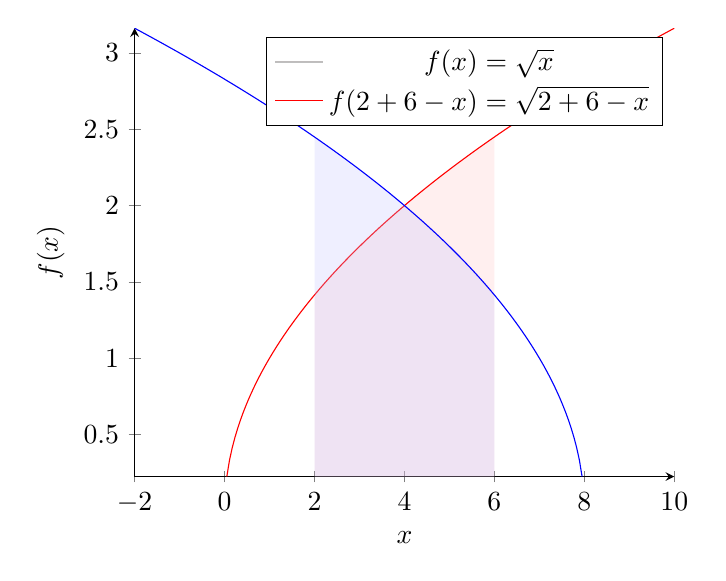
\begin{tikzpicture}
        \begin{axis}[
            axis lines = left,
            xlabel = $x$,
            ylabel = {$f(x)$},
        ]
        % yes please
        \addplot[
            draw = none,
            fill = red!25,
            opacity = 0.25,
            domain = 2:6,
        ] {(x)^(1/2)} \closedcycle;
        \addplot[
            domain = -2:10,
            samples = 200,
            color = red,
        ]{(x)^(1/2)};
        \addlegendentry{$f(x)=\sqrt{x}$}
        
        \addplot[
            draw = none,
            fill = blue!25,
            opacity = 0.25,
            domain = 2:6,
        ]{(8-x)^(1/2)} \closedcycle;
        \addplot[
            domain = -2:10,
            samples = 200,
            color = blue,
        ]{(8-x)^(1/2)};
        \addlegendentry{$f(2+6-x)=\sqrt{2+6-x}$}
            
        \end{axis}
    
    \end{tikzpicture}
    \caption{Graphical intuition behind $x\mapsto a+b-x$.}
    \label{fig:reflectionsubstitution}
\end{figure}

\noindent Using our substitution rule we know that 

\begin{align*}
    \int_2^6 \sqrt{x}\,\dx x &= \int_2^6 \sqrt{2+6-x}\,\dx x \\
    &= \left[ -\frac 2 3 (8-x)^{3/2} \right]_2^6 \\
    &= -\frac{2}{3} \left( 2\sqrt2-6\sqrt6 \right). 
\end{align*}

Now we can validate this by checking the original integral, which indeed is the same (\textit{you can check for yourself}).

\subsection*{Examples}

1. Evaluate $\displaystyle \int_0^\pi \frac{\sin^2x}{\pi-x}\,\dx x$

\begin{ExampleBody}
    The Reflection Substitution often comes in handy when $a=0$, $b=\pi$, and there's a sine function within the integrand. This is because $\sin(\pi-x) = \sin(x)$. This applies directly to the current problem.
    
    \begin{align}
        \int_0^\pi \frac{\sin^2 x}{\pi-x}\,\dx x &= \int_0^\pi \frac{\sin^2 x}{x}\,\dx x \label{eq:refsub1}\\
        &\approx 1.21883 \label{eq:refsub2}
    \end{align}
    In step (\ref{eq:refsub1}) we make the substitution $x\mapsto\pi-x$. On the next line, (\ref{eq:refsub2}), we use numeric approximations, because the resulting integral does not have an elementary anti-derivative.
\end{ExampleBody}

2. Evaluate $\displaystyle \int_0^\pi \frac{x\tan x}{\sec x + \cos x}\,\dx x$.

\begin{ExampleBody}
    Again, begin this by making the substitution $x\mapsto\pi-x$.
    \begin{align*}
        I &=\int_0^\pi     \frac{(\pi-x)\tan(\pi-x)}{\sec(\pi-x)+\cos(\pi-x)}\,\dx x\\ 
        &=\int_0^\pi     \frac{(x-\pi)(-\tan(x))}{-\sec(x)-\cos(x)}\,\dx x\\ 
        &= \pi\int_0^\pi\frac{\tan(x)}{\sec(x)+\cos(x)}\,\dx x-I
    \end{align*}
    Let $J = \int_0^\pi \frac{\tan(x)}{\sec(x)+\cos(x)}\,\dx x$, such that $I = \frac{\pi}{2} J$. We can find $J$ by substituting $u\mapsto\cos x$ and we get $J=\frac{\pi}{2}$. Substituting back in,
    
    $$ I = \frac{\pi}{2} J = \frac{\pi^2}{4} .$$
    
\end{ExampleBody}


\subsection*{Exercises}

\begin{enumerate}

    \item Show that $\displaystyle \int_0^\pi xf(\sin x)\,\dx x = \frac{\pi}{2}\int_0^\pi f(\sin x)\,\dx x$. \  \hint{$\sin(\pi - x) = \sin x$}
    \item Show that $\displaystyle \int_0^{n\pi}f(\cos^2\theta)\,\dx \theta = n\int_0^\pi f(\cos^2\theta)\,\dx \theta$.
\end{enumerate}